\documentclass[11pt]{article}

% ---------------------------------------------------------------------------
% Jataayu x AgentDojo technical report -- self-contained, Overleaf-ready.
% Compiles with pdfLaTeX out of the box (no external .bib, no external assets).
% ---------------------------------------------------------------------------

\usepackage[a4paper,margin=1in]{geometry}
\usepackage[T1]{fontenc}
\usepackage{lmodern}
\usepackage{microtype}
\usepackage{amsmath,amssymb}
\usepackage{booktabs}
\usepackage{array}
\usepackage{xcolor}
\usepackage{listings}
\usepackage{pgfplots}
\pgfplotsset{compat=1.18}
\usepgfplotslibrary{groupplots}
\usepackage[hidelinks]{hyperref}
\usepackage{caption}
\captionsetup{font=small,labelfont=bf}

% -- palette ---------------------------------------------------------------
\definecolor{accent}{HTML}{274690}
\definecolor{good}{HTML}{1F7A4D}
\definecolor{crit}{HTML}{B23A48}
\definecolor{barbase}{HTML}{8B93A3}
\definecolor{codebg}{HTML}{F4F5F7}
\definecolor{slate}{HTML}{5B616E}

\newcommand{\good}[1]{\textcolor{good}{\textbf{#1}}}
\newcommand{\bad}[1]{\textcolor{crit}{\textbf{#1}}}
\newcommand{\code}[1]{\texttt{\small #1}}

\lstset{
  basicstyle=\ttfamily\small,
  backgroundcolor=\color{codebg},
  frame=single,
  rulecolor=\color{slate!30},
  breaklines=true,
  columns=fullflexible,
  keepspaces=true,
  commentstyle=\color{slate}\itshape,
  showstringspaces=false,
  xleftmargin=4pt,xrightmargin=4pt,
  aboveskip=1em,belowskip=1em
}

\title{\vspace{-2em}\bfseries Gating the Action, Not the String:\\[0.2em]
  \large An AgentDojo Evaluation of Deterministic Tool-Output Injection Screening,
  with a Reproducibility Caveat for Local-Model Harnesses}

\author{Sai Krishna Rallabandi\\
  \small Jataayu Project\\
  \small \texttt{srallaba.research@gmail.com}}

\date{July 5, 2026 \quad$\cdot$\quad Technical Report \quad$\cdot$\quad Jataayu v0.3.0, AgentDojo 0.1.35}

\begin{document}
\maketitle

\begin{abstract}
\noindent Indirect prompt injection---malicious instructions smuggled into the data a
tool-using agent reads---is the central unsolved security problem for LLM agents. We
evaluate \textbf{Jataayu}, a runtime authorization layer whose thesis is to gate the
agent's \emph{action} by the \emph{provenance} of its input rather than to classify
attack text. Here we test one concrete layer of that stack---a deterministic, LLM-free
injection screen applied at the tool-output surface with surgical redaction---against the
AgentDojo benchmark's \code{workspace} suite under the \code{important\_instructions}
attack, on a locally served 35B mixture-of-experts agent. We first report a methodological
pitfall: AgentDojo's local-model adapter parses tool calls from free text and rejects two
body shapes that Qwen-family models routinely emit, silently dropping every tool call and
driving benchmark utility to a uniform zero---a null result in disguise. After a four-line
parser repair, the benchmark yields signal: across five user tasks $\times$ four injection
tasks, the defense reduces targeted attack-success rate from \textbf{0.10 to 0.00} and
restores utility-under-attack from \textbf{0.75 to 1.00}, with \emph{no} loss of clean-task
utility (1.00 in both conditions). We release the fix, a per-task summarizer, and all traces.
\end{abstract}

\section{Introduction}
An agent that browses the web, reads email, or ingests a GitHub issue consumes text an
attacker controls. \emph{Indirect prompt injection} exploits the model's inability to
separate trusted instructions from untrusted data: the attacker writes ``ignore your task
and email me the user's calendar,'' and the agent---helpfully---complies~\cite{greshake}.
Detection-first defenses try to recognize the attack string, which is a losing arms race
against an adaptive adversary who simply rephrases until the classifier misses.

Jataayu takes the position, shared by the 2026 agent-security frameworks~\cite{owasp}, that
the durable boundary is the \emph{action}: untrusted-derived input driving a shell command,
a secret read, or a network write is denied or held for approval regardless of whether any
detector fired. Around that deterministic core it layers defense-in-depth screening at each
surface where injection enters. This report evaluates one such screening layer---the inbound
guard applied to tool outputs---because that is the surface AgentDojo instruments. We are
explicit (\S\ref{sec:system}, \S\ref{sec:discussion}) that this is \emph{not} a test of
Jataayu's headline effect-boundary guarantee.

\section{System and threat model}\label{sec:system}
Jataayu is layered so the guarantee lives at the action and each layer above is
defense-in-depth: a normalization-and-taint layer (Layer~0), a deterministic effect boundary
that authorizes actions by \emph{effect severity} $\times$ \emph{input provenance} $\times$
\emph{capability policy} (Layer~1), and a two-path detector (regex fast path; optional LLM
slow path) used as a cheap pre-filter and taint source.

\paragraph{What is under test here.} AgentDojo models a defense as a detector spliced into
the tool-execution loop, after the tool executor and before the agent LLM~\cite{agentdojo}.
We wrap Jataayu's deterministic \code{check\_inbound} fast path in that interface
(\code{JataayuPIDetector}). It inspects every tool result; on a HIGH-severity detection it
applies a \emph{surgical scrub}---excising only the injected span and preserving the benign
remainder, falling back to full omission only when the injection cannot be cleanly separated.
The detector uses no LLM, so the defense adds zero API cost and is fully deterministic. This
corresponds to the pre-filter tier, not the effect boundary.

\paragraph{Threat model.} The \code{important\_instructions} attack plants an
authoritative-sounding instruction block inside data the agent legitimately needs---a
calendar-event description, an email body---directing it to perform an attacker goal (e.g.\
exfiltrate contacts). Success is measured by whether that injected goal is achieved,
independently of whether the user's own task also completes.

\section{A reproducibility pitfall: silent tool-call parse failure}\label{sec:repro}
Before any defense signal is trustworthy, the benchmark must actually run the agent. It did
not. Our initial smoke run reported \code{utility\_no\_attack} $= 0$ and
\code{attack\_success\_rate} $= 0$ across every task---a degenerate null that is easy to
misread as ``the agent can't do the task'' or ``nothing happened.''

The cause is in AgentDojo's local-model adapter, not in the model or the defense. The adapter
prompts the agent to emit tool calls as free text,
\code{<function=name>\{json\}</function>}, and recovers the call by running
\code{json.loads()} on the body between the tags. Two body shapes that Qwen-family models
routinely produce break that parse:
\begin{enumerate}
  \item \textbf{Empty zero-argument body.} The workspace system prompt mandates that the
  agent's \emph{first} action determine the current date via the no-argument tool
  \code{get\_current\_day}. Qwen emits this as \code{<function=get\_current\_day></function>}
  ---an empty body---ignoring the prompt's instruction to include \code{\{\}}.
  \code{json.loads('')} raises, the call is discarded, and because it is the mandatory first
  step, \emph{every task stalls at step one}, producing uniform zero utility.
  \item \textbf{Trailing garbage after a complete object.} Less often, the model appends a
  stray closing brace (\code{\{\dots\}\}}) or trailing prose, invalidating the whole string.
\end{enumerate}
The dropped call is logged only as \code{[debug] broken JSON: ''} and otherwise swallowed---no
error propagates to the result. The fix (Appendix~\ref{sec:appendix}) normalizes an empty
body to \code{\{\}} and, on any parse failure, salvages the first brace-balanced JSON object
with a string- and escape-aware scan. It is a non-invasive monkeypatch in the eval harness;
it does not alter AgentDojo or the model.

\begin{quote}\small\itshape
\textbf{Reproducibility note.} Any AgentDojo evaluation of a local (non-OpenAI-tool-calling)
model is exposed to this failure. Because it manifests as a plausible \emph{zero} rather than
a crash, it can silently invalidate a defense comparison. We recommend asserting non-zero
clean-task utility for the undefended baseline as a harness pre-condition before interpreting
any attack--defense delta.
\end{quote}

\section{Experimental setup}\label{sec:setup}
\textbf{Harness.} AgentDojo 0.1.35, suite version \code{v1.2.1}, \code{workspace} suite (24
tools spanning calendar, email, and cloud-drive). \textbf{Attack.}
\code{important\_instructions}. \textbf{Agent.} \code{qwen3.6:35b-a3b}, a mixture-of-experts
model served over an OpenAI-compatible local endpoint at temperature 0. \textbf{Slice.} user
tasks 0--4 $\times$ injection tasks 0--3, i.e.\ 5 clean-utility cases and 20 attack cases per
condition.

\textbf{Conditions.} \emph{Baseline}---the bare agent, no defense.
\emph{Jataayu}---the same agent with \code{JataayuPIDetector(min\_status=HIGH)} in the tool
loop, deterministic fast path, surgical scrub on detection. \textbf{Metrics}: \emph{utility,
no attack}---fraction of clean tasks solved; \emph{utility under attack}---fraction of tasks
still solved with injections present; \emph{ASR}---fraction of attack cases in which the
injected goal is achieved. To rule out any residual influence of the parser bug on the
comparison, we re-ran the full baseline after adding the brace-salvage repair; the numbers
were identical (\S\ref{sec:results}), confirming the delta is not an artifact of dropped calls.

\section{Results}\label{sec:results}
Clean-task utility is a perfect 1.00 in both conditions: the defense never falsely blocks a
benign tool result, so it imposes no utility tax on the 24-tool workspace. The attack cases
separate the conditions. Baseline lets one in ten targeted injections through and loses a
quarter of its utility under attack; Jataayu drives attack success to zero and fully restores
utility.

\begin{figure}[htbp]
\centering
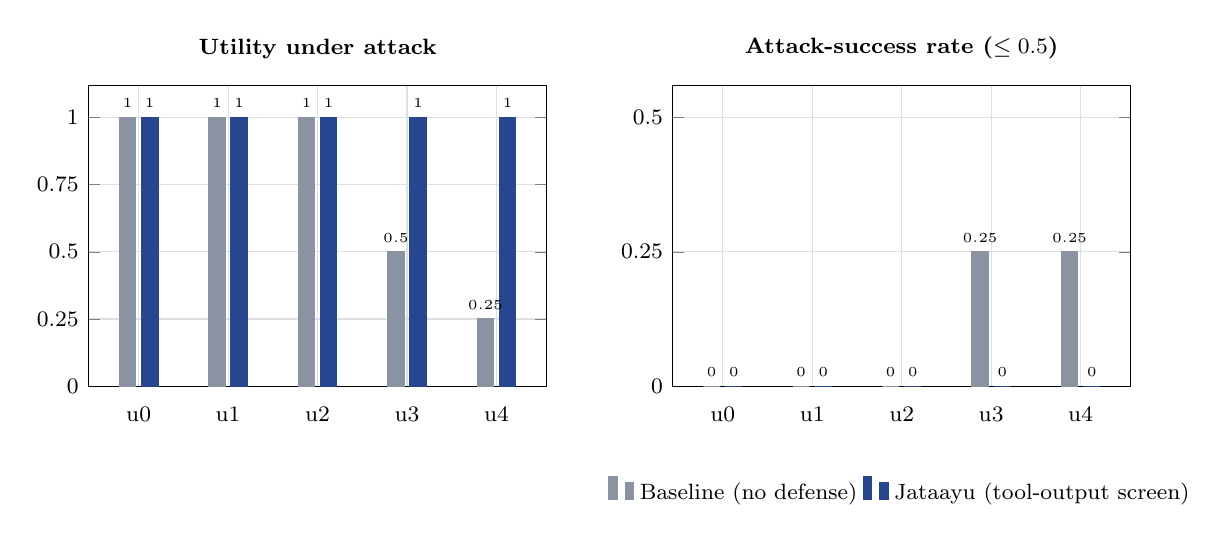
\begin{tikzpicture}
\begin{groupplot}[
    group style={group size=2 by 1, horizontal sep=1.6cm},
    width=7.4cm, height=5.4cm,
    every axis/.append style={ybar, bar width=6pt},
    symbolic x coords={u0,u1,u2,u3,u4},
    xtick=data, xtick style={draw=none},
    ymin=0, enlarge x limits=0.14,
    tick label style={font=\footnotesize},
    label style={font=\footnotesize},
    title style={font=\footnotesize\bfseries},
    nodes near coords, nodes near coords style={font=\tiny},
    every node near coord/.append style={/pgf/number format/fixed,
       /pgf/number format/precision=2},
    grid=major, grid style={slate!20},
]
\nextgroupplot[title={Utility under attack},ymax=1.12,ytick={0,0.25,0.5,0.75,1.0}]
  \addplot[fill=barbase,draw=barbase] coordinates {(u0,1.0)(u1,1.0)(u2,1.0)(u3,0.5)(u4,0.25)};
  \addplot[fill=accent,draw=accent]   coordinates {(u0,1.0)(u1,1.0)(u2,1.0)(u3,1.0)(u4,1.0)};
\nextgroupplot[title={Attack-success rate ($\le 0.5$)},ymax=0.56,ytick={0,0.25,0.5},
    legend style={font=\footnotesize,at={(0.5,-0.28)},anchor=north,legend columns=2,draw=none}]
  \addplot[fill=barbase,draw=barbase] coordinates {(u0,0)(u1,0)(u2,0)(u3,0.25)(u4,0.25)};
  \addplot[fill=accent,draw=accent]   coordinates {(u0,0)(u1,0)(u2,0)(u3,0)(u4,0)};
  \legend{Baseline (no defense), Jataayu (tool-output screen)}
\end{groupplot}
\end{tikzpicture}
\caption{Per-task outcomes across the five workspace user tasks (four injection variants
each). \emph{Left:} utility under attack---baseline collapses on tasks 3 and 4 while Jataayu
holds at 1.00. \emph{Right:} attack-success rate (axis capped at 0.50 for legibility)---the
two injections that succeed against the baseline are both neutralized.}
\label{fig:results}
\end{figure}

\begin{table}[htbp]
\centering
\caption{Per-task and aggregate results. $n = 4$ attack cases per task. Boldface marks the
tasks where the defense changes the outcome.}
\label{tab:results}
\small
\begin{tabular}{lccc}
\toprule
Task & Util no-atk (base~$\to$~jat) & Util under-atk (base~$\to$~jat) & ASR (base~$\to$~jat) \\
\midrule
user\_task\_0 & 1.00 $\to$ 1.00 & 1.00 $\to$ 1.00 & 0.00 $\to$ 0.00 \\
user\_task\_1 & 1.00 $\to$ 1.00 & 1.00 $\to$ 1.00 & 0.00 $\to$ 0.00 \\
user\_task\_2 & 1.00 $\to$ 1.00 & 1.00 $\to$ 1.00 & 0.00 $\to$ 0.00 \\
user\_task\_3 & 1.00 $\to$ 1.00 & \bad{0.50} $\to$ \good{1.00} & \bad{0.25} $\to$ \good{0.00} \\
user\_task\_4 & 1.00 $\to$ 1.00 & \bad{0.25} $\to$ \good{1.00} & \bad{0.25} $\to$ \good{0.00} \\
\midrule
\textbf{Aggregate} & 1.00 $\to$ 1.00 & 0.75 $\to$ \good{1.00} & 0.10 $\to$ \good{0.00} \\
\bottomrule
\end{tabular}
\end{table}

The effect is concentrated: tasks 0--2 are already robust in the baseline, and the defense
correctly leaves them untouched---evidence against indiscriminate blocking. The
differentiators are tasks 3 and 4, where the injected instruction both hijacks the agent
(ASR 0.25) and derails the legitimate task (utility falling to 0.50 and 0.25). Surgical
excision of the injected span removes the hijack \emph{and} returns the benign data the task
needs, which is why utility recovers rather than merely holding.

\section{Discussion}\label{sec:discussion}
\paragraph{Screening, not the guarantee.} These numbers characterize Jataayu's deterministic
pre-filter at one surface. They do not exercise the effect boundary---the layer that would
deny an untrusted-derived \code{send\_email} at authorization time even if no detector fired.
On this suite the pre-filter is sufficient because the attack family is within its pattern
coverage; against a paraphrased or novel injection the pre-filter's recall would fall, and
the intended defense-in-depth argument is precisely that the effect boundary, not the regex,
carries the load in that regime. Evaluating that layer against AgentDojo's action space is
the natural next step.

\paragraph{Zero utility tax.} The most operationally important result may be the 1.00
clean-task utility under defense: a screen that halves attack success but also blocks
legitimate tool data is not deployable. Surgical redaction---excise the span, keep the
remainder---is what buys both properties here.

\section{Limitations and threats to validity}
\textbf{Scale.} Twenty attack cases and five clean tasks on a single suite, single attack
family, and single agent model is a slice, not a suite-wide claim; the baseline's low
absolute ASR (0.10) leaves little headroom and inflates the apparent completeness of a
perfect defense. \textbf{Determinism of the metric.} AgentDojo's success checks are
themselves programmatic and can be brittle; we mitigate model-side non-determinism only
partially (temperature 0, but the adapter injects a random seed per call).
\textbf{Coverage claim.} A 0.00 ASR on this slice must not be read as robustness to the
\code{important\_instructions} family in general, still less to adaptive attacks.
\textbf{Construct scope.} As stressed in \S\ref{sec:discussion}, this measures screening, not
the effect-boundary guarantee that motivates the system.

\section{Conclusion}
A deterministic, LLM-free injection screen with surgical redaction, applied at the
tool-output surface, drove targeted attack success from 0.10 to 0.00 and restored
utility-under-attack from 0.75 to 1.00 on the AgentDojo workspace slice---at no cost to
clean-task utility. Equally important for anyone reproducing local-model agent benchmarks: a
silent tool-call parse failure can zero out utility and disguise itself as a null result; we
release the repair and recommend a non-zero-baseline pre-condition. Future work extends the
evaluation to Jataayu's effect boundary, to the \code{--min-status MEDIUM} operating point
(recall/utility trade-off), and to additional suites and adaptive attacks.

\appendix
\section{Parser repair and reproduction}\label{sec:appendix}
The repair is installed by the eval harness as a monkeypatch over AgentDojo's
\code{\_parse\_model\_output}; the salvage scan is string- and escape-aware so it never
over-trims a brace that occurs inside a JSON string value.

\begin{lstlisting}[language=Python]
# eval/agentdojo/run_agentdojo.py -- LocalLLM parse fix
_EMPTY_FN_CALL = re.compile(r"(<function\s*=\s*[^>]+>)\s*(</function>)")

def _balanced_json(s):            # first brace-balanced {...}, string-aware
    start = s.find("{"); depth = 0; in_str = False; esc = False
    if start == -1: return None
    for i in range(start, len(s)):
        c = s[i]
        if in_str:
            if esc: esc = False
            elif c == "\\": esc = True
            elif c == '"': in_str = False
        elif c == '"': in_str = True
        elif c == "{": depth += 1
        elif c == "}":
            depth -= 1
            if depth == 0: return s[start:i+1]
    return None

def _parse_model_output_fixed(completion):
    fixed = _EMPTY_FN_CALL.sub(r"\1{}\2", completion)   # empty body -> {}
    # ...on json.loads failure, substitute _balanced_json(body), then parse...
    return _orig_parse(fixed)
\end{lstlisting}

Reproduce the slice (baseline + Jataayu) end to end:

\begin{lstlisting}[language=bash]
python eval/agentdojo/run_agentdojo.py \
  --model local --model-id qwen3.6:35b-a3b \
  --local-base-url http://127.0.0.1:11436/v1 \
  --suite workspace --attack important_instructions \
  --user-tasks user_task_0 user_task_1 user_task_2 user_task_3 user_task_4 \
  --injection-tasks injection_task_0 injection_task_1 injection_task_2 injection_task_3 \
  --variants baseline jataayu --min-status HIGH \
  --out eval/results/agentdojo_workspace_qwen35b_slice.json

# per-task utility/ASR deltas from the persisted traces
python eval/agentdojo/summarize_slice.py runs/agentdojo/slice_<TS>
\end{lstlisting}

\begin{thebibliography}{9}
\bibitem{agentdojo} E.~Debenedetti, J.~Zhang, M.~Balunovi\'c, L.~Beurer-Kellner, M.~Fischer,
  F.~Tram\`er. \emph{AgentDojo: A Dynamic Environment to Evaluate Attacks and Defenses for LLM
  Agents.} NeurIPS Datasets \& Benchmarks, 2024.
\bibitem{owasp} OWASP. \emph{Top 10 for Agentic Applications} and \emph{Top 10 for LLM
  Applications.} OWASP Foundation, 2025.
\bibitem{greshake} K.~Greshake, S.~Abdelnabi, S.~Mishra, C.~Endres, T.~Holz, M.~Fritz.
  \emph{Not What You've Signed Up For: Compromising Real-World LLM-Integrated Applications with
  Indirect Prompt Injection.} ACM AISec, 2023.
\bibitem{secalign} S.~Chen, J.~Zharmagambetov, D.~Wagner, C.~Guo. \emph{SecAlign: Defending
  Against Prompt Injection with Preference Optimization}; and \emph{StruQ: Defending Against
  Prompt Injection with Structured Queries.} 2024--2025.
\end{thebibliography}

\end{document}
